\section{Utilizzo degli spazi nel chiosco interno ed esterno}

\begin{figure}[H]
	\centering
	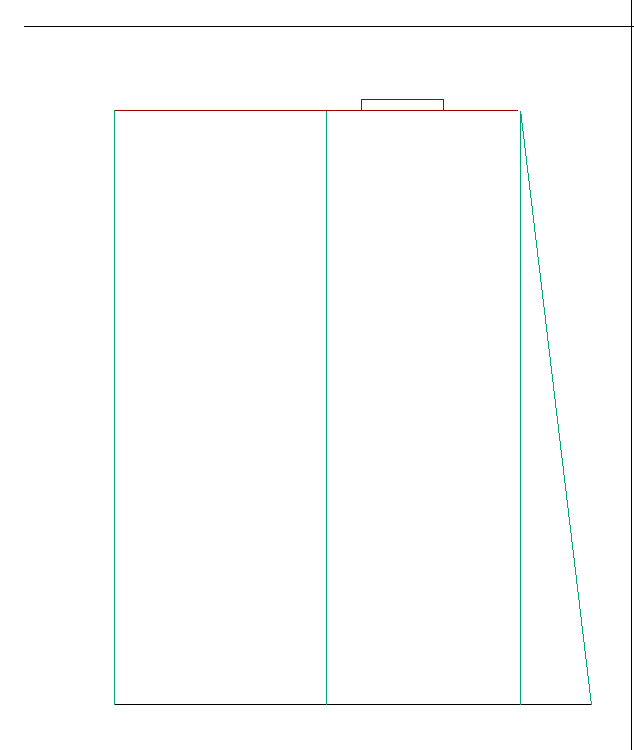
\includegraphics[width=0.5\textwidth]{image42}
	\caption{Vista struttura}
	\label{fig:mesh1}
\end{figure}


\begin{figure}[H]
	\centering
	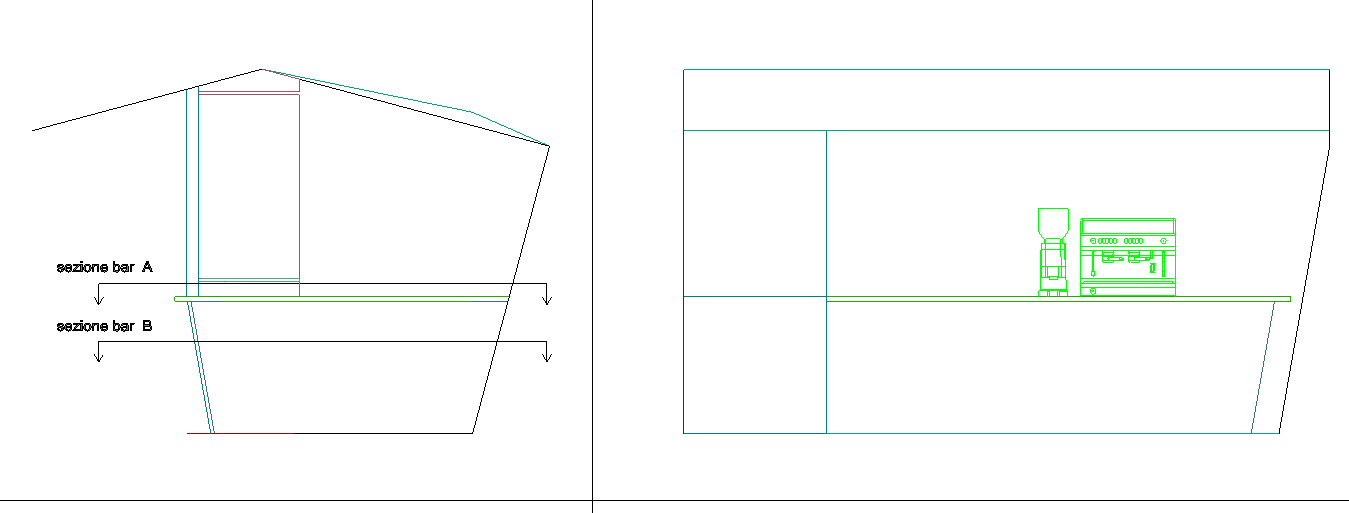
\includegraphics[width=0.8\textwidth]{image23}
	\caption{aaa}
	\label{fig:mesh1}
\end{figure}


\subsection{Progettazione bancone}


\begin{figure}[H]
	\centering
	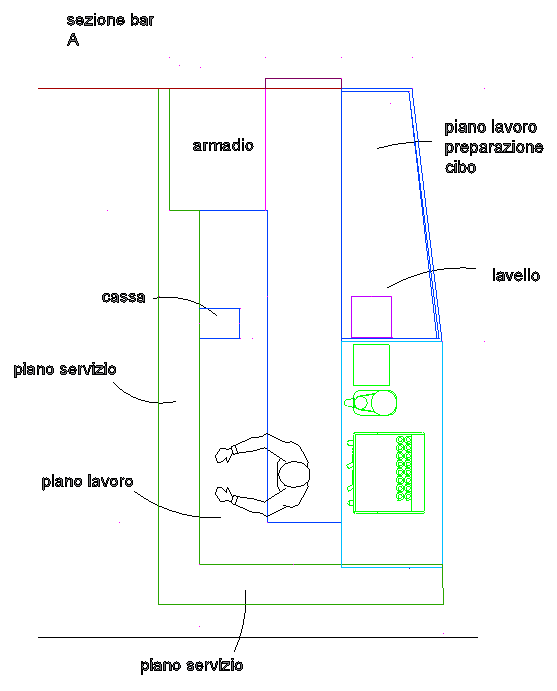
\includegraphics[width=0.5\textwidth]{image29}
	\caption{Progettazione bancone}
	\label{fig:mesh1}
\end{figure}

Nell'immagine  possiamo vedere la composizione del bar  , dove troviamo un'area di lavoro divisa in due. La parte di ordini/cassa e preparazione del cibo  e la parte caffetteria/ distribuzione bibite.

\begin{figure}[H]
	\centering
	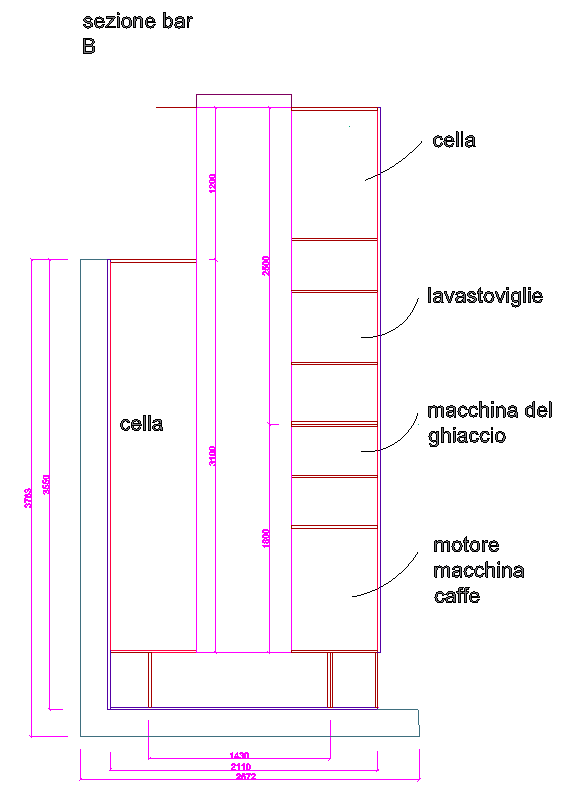
\includegraphics[width=0.5\textwidth]{image13}
	\caption{Sezione bar B}
	\label{fig:mesh1}
\end{figure}

sezione B
Qui possiamo vedere come ho gestito la divisione dei moduli.
Sul lato sinistro troviamo un armadio da 1200 mm e uno spazio dove collocare una cella da 3000 mm .
Sul lato opposto troviamo un modulo dalla lunghezza totale di 4300 mm 
Uan  altro piccolo modulo di 1430mm disposto perpendicolare a questi due chiude la zona lavoro. 

\begin{figure}[H]
	\centering
	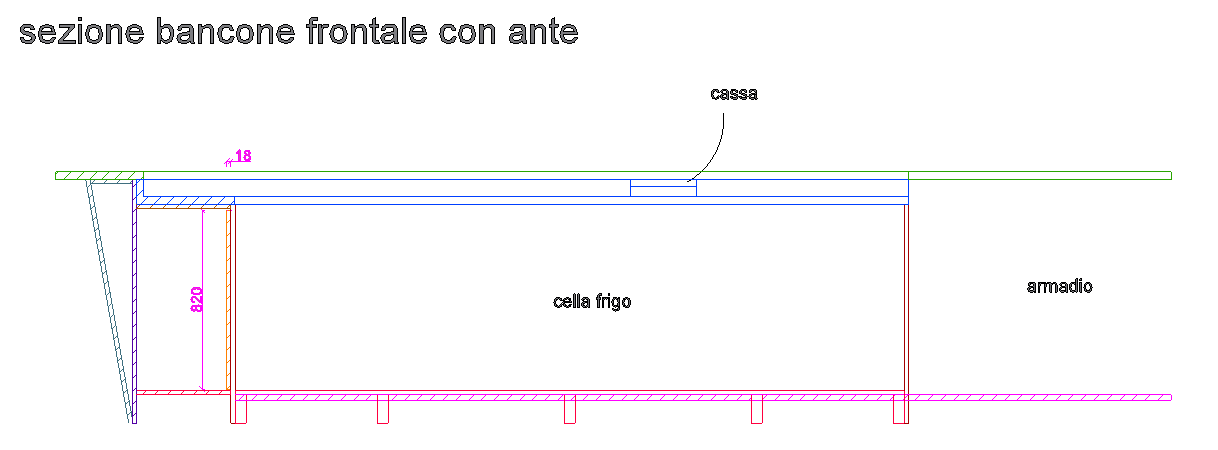
\includegraphics[width=0.8\textwidth]{image4}
	\caption{Sezione bancone frontale con ante}
	\label{fig:mesh1}
\end{figure}


Possiamo vedere in verde le misure del bancone di servizio ed in blu il piano di lavoro dove è anche collocata la  cassa  ed in fine il vano per la cella dalla lunghezza di 3000 mm . 
Il vano a destra è riservato alla collocazione di un armadio su misura. 

\begin{figure}[H]
	\centering
	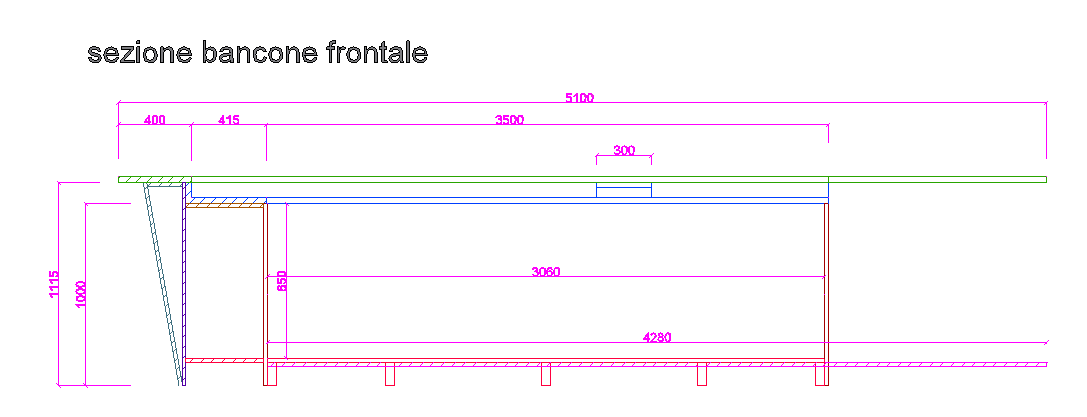
\includegraphics[width=0.8\textwidth]{image20}
	\caption{Sezione bancone frontale}
	\label{fig:mesh1}
\end{figure}

\begin{figure}[H]
	\centering
	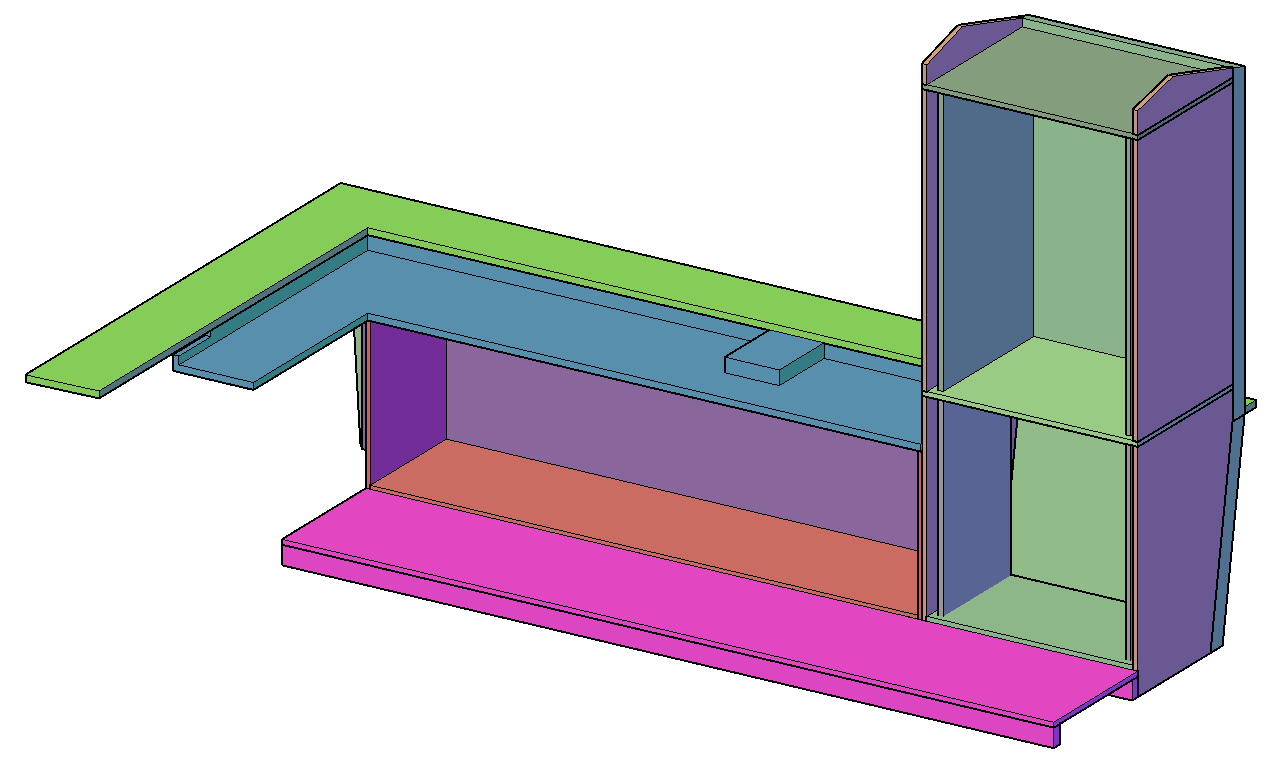
\includegraphics[width=0.8\textwidth]{image26}
	\caption{Sezione bar A}
	\label{fig:mesh1}
\end{figure}

Il primo modulo da $2500mm$ contiene una cella da $1000 mm$, un piccolo armadietto, un vano riservato alla lavastoviglie, un altro piccolo armadietto e il vano dove sarà inserito il lavello.

\begin{figure}[H]
	\centering
	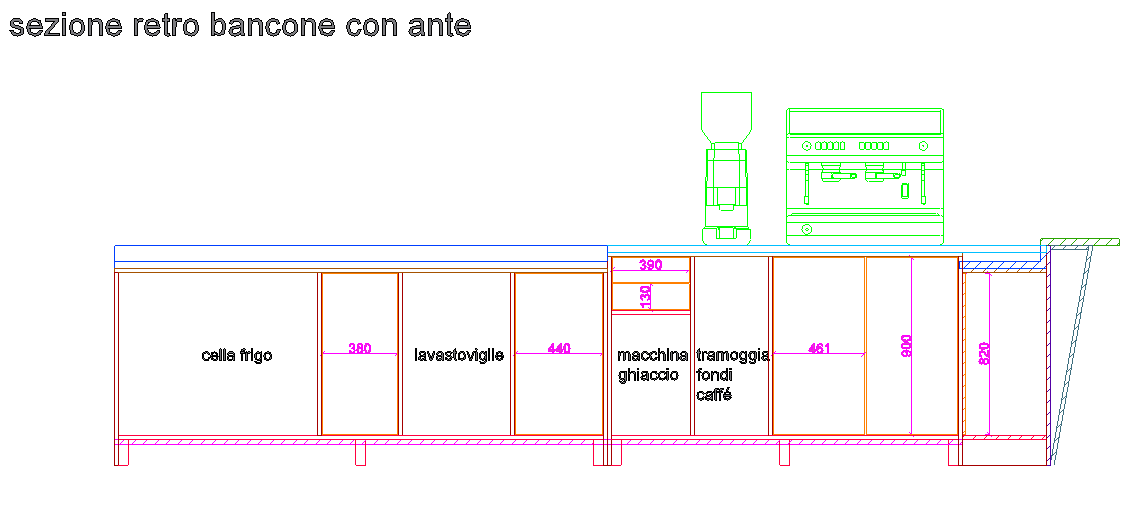
\includegraphics[width=0.8\textwidth]{image41}
	\caption{???}
	\label{fig:mesh1}
\end{figure}

Il secondo modulo da $1800 mm$ contiene un vano con cassetti e la macchina per il ghiaccio ,un vano tramoggia fondi caffè e spazzatura ed un armadietto a due ante dove è collocata la pompa per la macchina del caffè.

\begin{figure}[H]
	\centering
	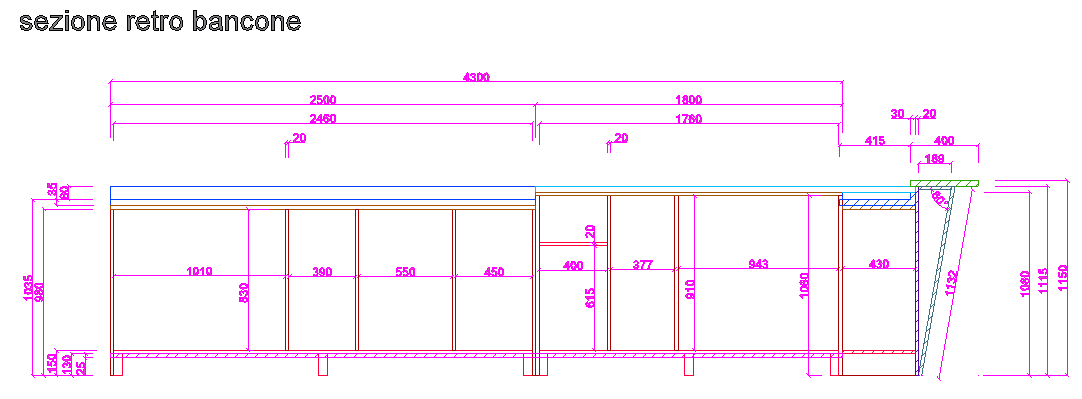
\includegraphics[width=0.8\textwidth]{image10}
	\caption{Sezione retro bancone}
	\label{fig:mesh1}
\end{figure}
\begin{figure}[H]
	\centering
	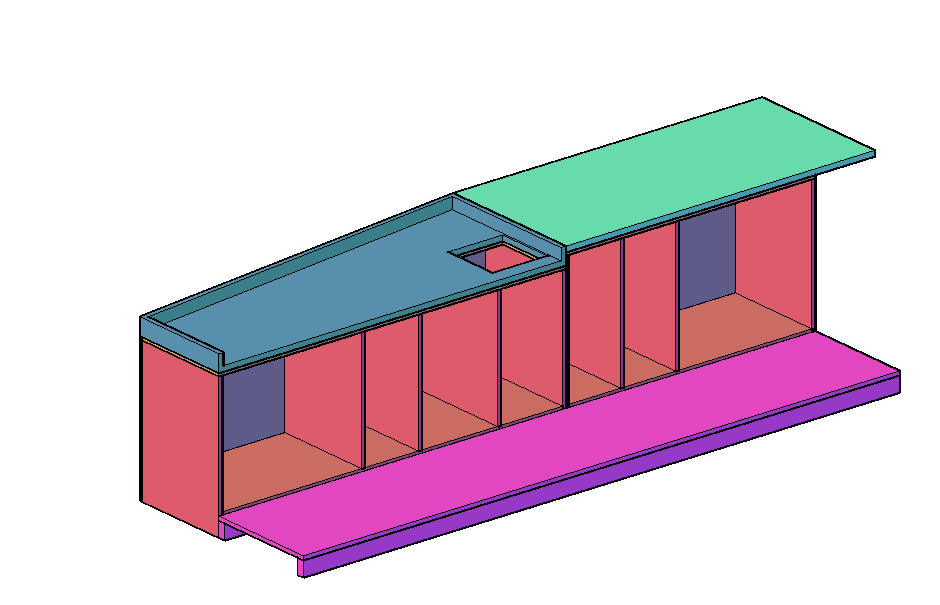
\includegraphics[width=0.8\textwidth]{image7}
	\caption{aaaa}
	\label{fig:mesh1}
\end{figure}
\begin{figure}[H]
	\centering
	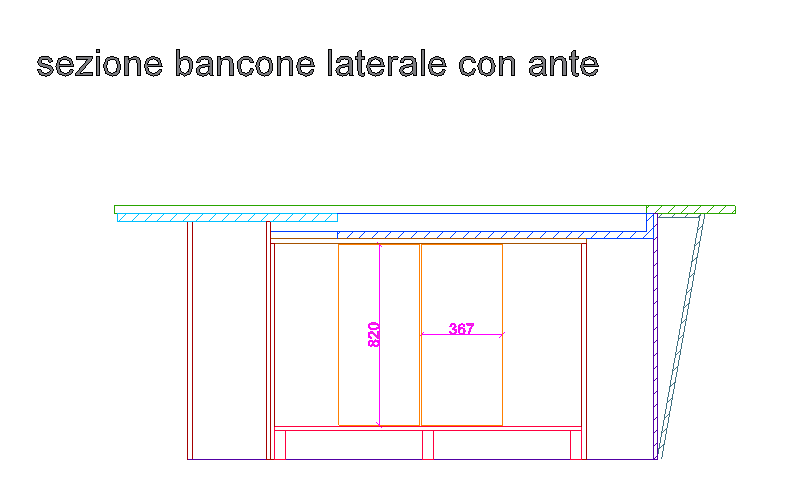
\includegraphics[width=0.8\textwidth]{image37}
	\caption{Sezione bancone laterale con ante}
	\label{fig:mesh1}
\end{figure}
\begin{figure}[H]
	\centering
	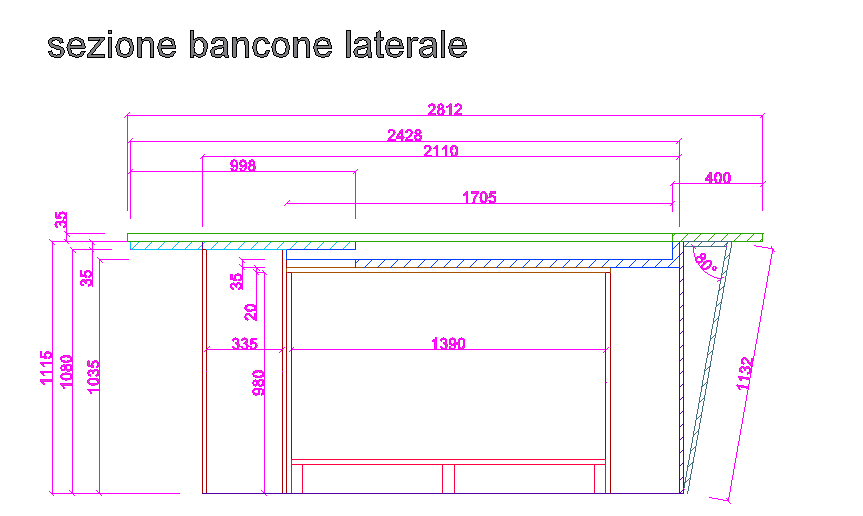
\includegraphics[width=0.8\textwidth]{image15}
	\caption{Sezione bancone laterale}
	\label{fig:mesh1}
\end{figure}
\begin{figure}[H]
	\centering
	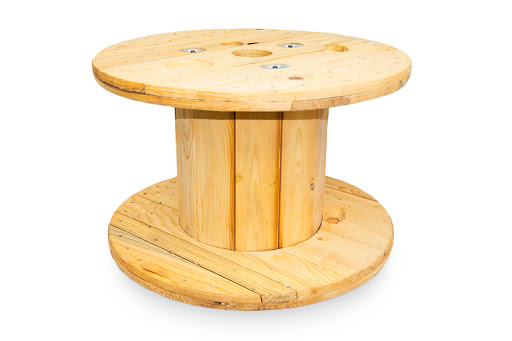
\includegraphics[width=0.8\textwidth]{image3}
	\caption{???}
	\label{fig:mesh1}
\end{figure}

\begin{figure}[H]
	\centering
	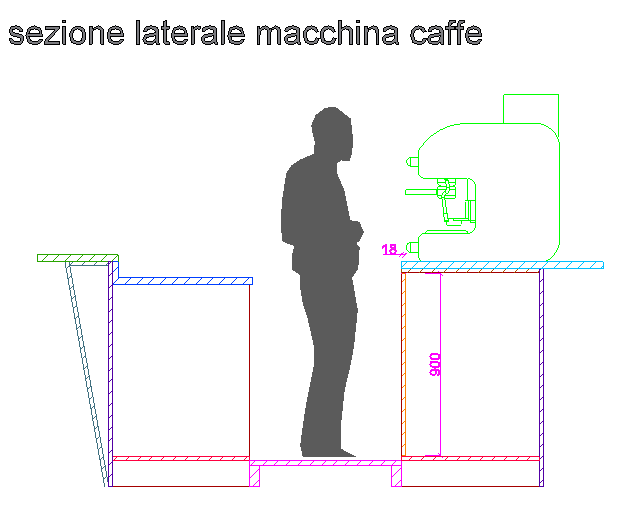
\includegraphics[width=0.8\textwidth]{image16}
	\caption{Sezione laterale macchina caffè}
	\label{fig:mesh1}
\end{figure}
\begin{figure}[H]
	\centering
	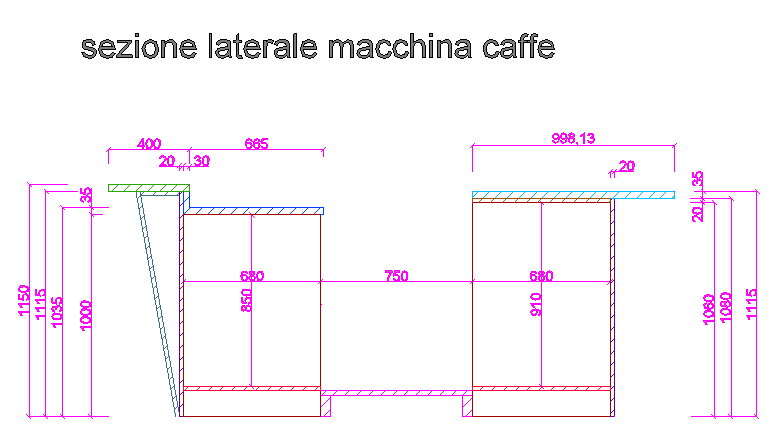
\includegraphics[width=0.8\textwidth]{image22}
	\caption{Sezione laterale macchina caffè}
	\label{fig:mesh1}
\end{figure}

\begin{figure}[H]
	\centering
	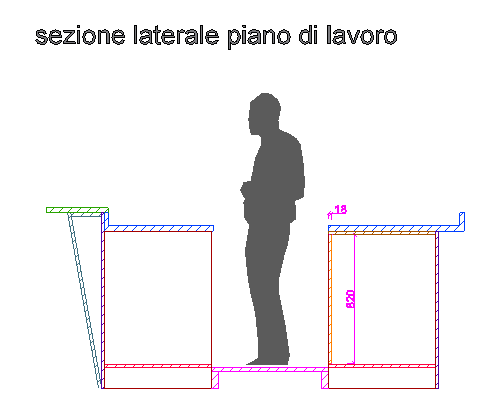
\includegraphics[width=0.8\textwidth]{image25}
	\caption{Sezione laterale piano di lavoro}
	\label{fig:mesh1}
\end{figure}

L’armadio ha una larghezza totale di 1200 mm, altezza di 3061 mm ed ha  una luce interna di 1020 mm. E’ composto da  due pezzi, una parte bassa dove troviamo il fondo in luce e il cappello che fa da fondo per la parte in alto. 
Le spalle sono composte da un fianco interno ed uno esterno. 
Come sistema di chiusura ho pensato ad un sistema a serranda orizzontale. 
Il materiale usato è multistrato  $25mm$.

\begin{figure}[H]
	\captionsetup[subfloat]{farskip=2pt,captionskip=8pt}
	\centering
	\subfloat[Vista armadio 3D]{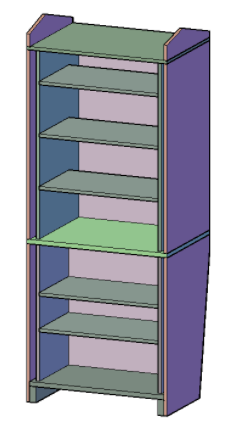
\includegraphics[width=4cm]{image57}}
	\hspace{1cm}
	\subfloat[Vista armadio]{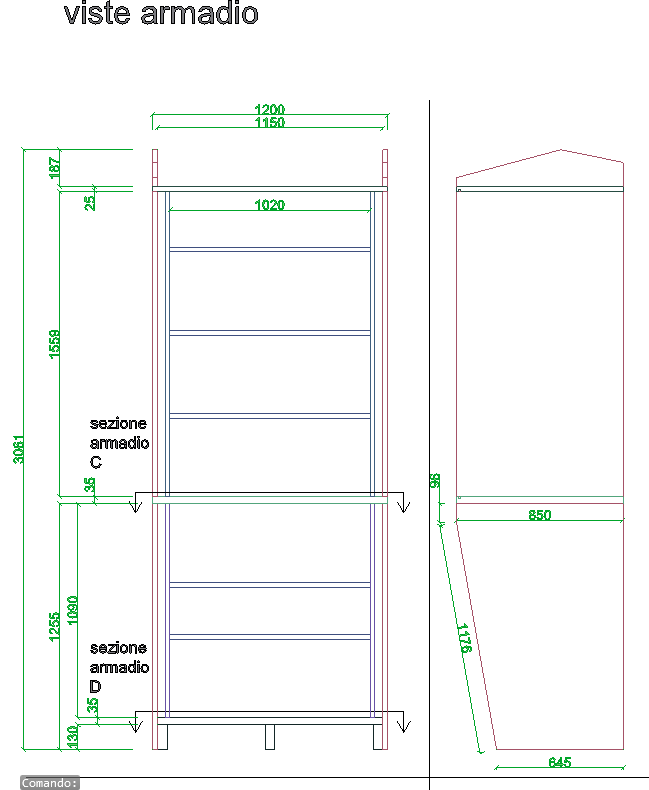
\includegraphics[width=6cm]{image19}}
	
	\caption{Armadio (sezione e vista 3D)}
	\label{fig:imagesizes}
\end{figure}

\begin{figure}[H]
	\captionsetup[subfloat]{farskip=2pt,captionskip=8pt}
	\centering
	\subfloat[Sezione laterale armadio]{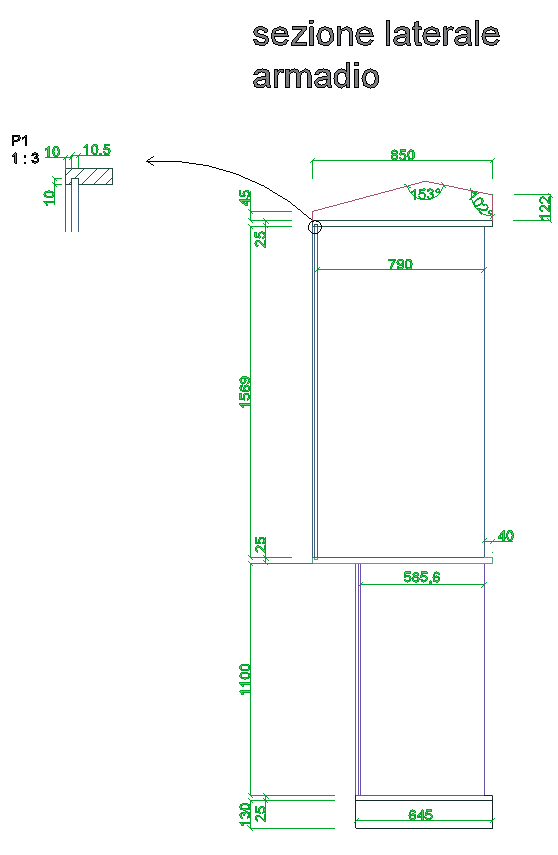
\includegraphics[width=4cm]{image6}}
	\hspace{1cm}
	\subfloat[Sezione armadio]{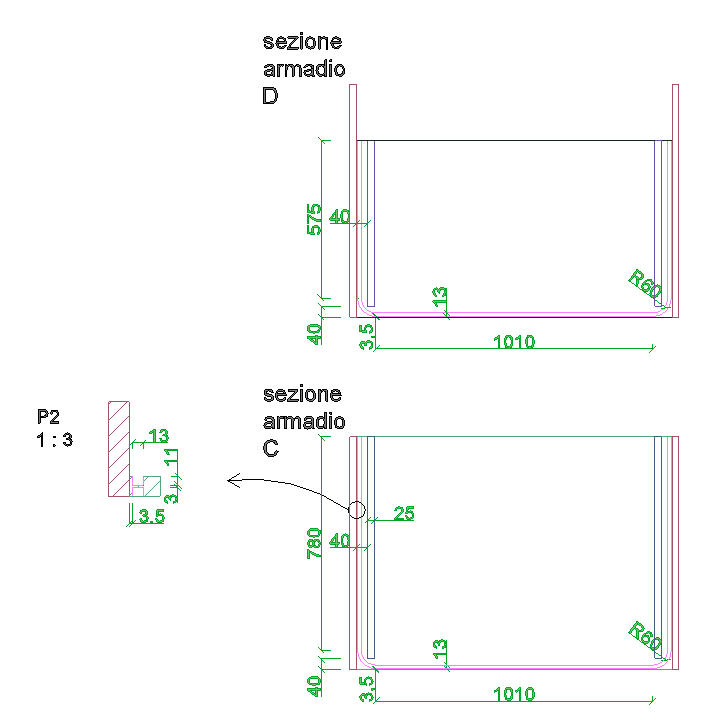
\includegraphics[width=6cm]{image30}}
	
	\caption{Sezione armadio}
	\label{fig:imagesizes}
\end{figure}


\begin{figure}[H]
	\centering
	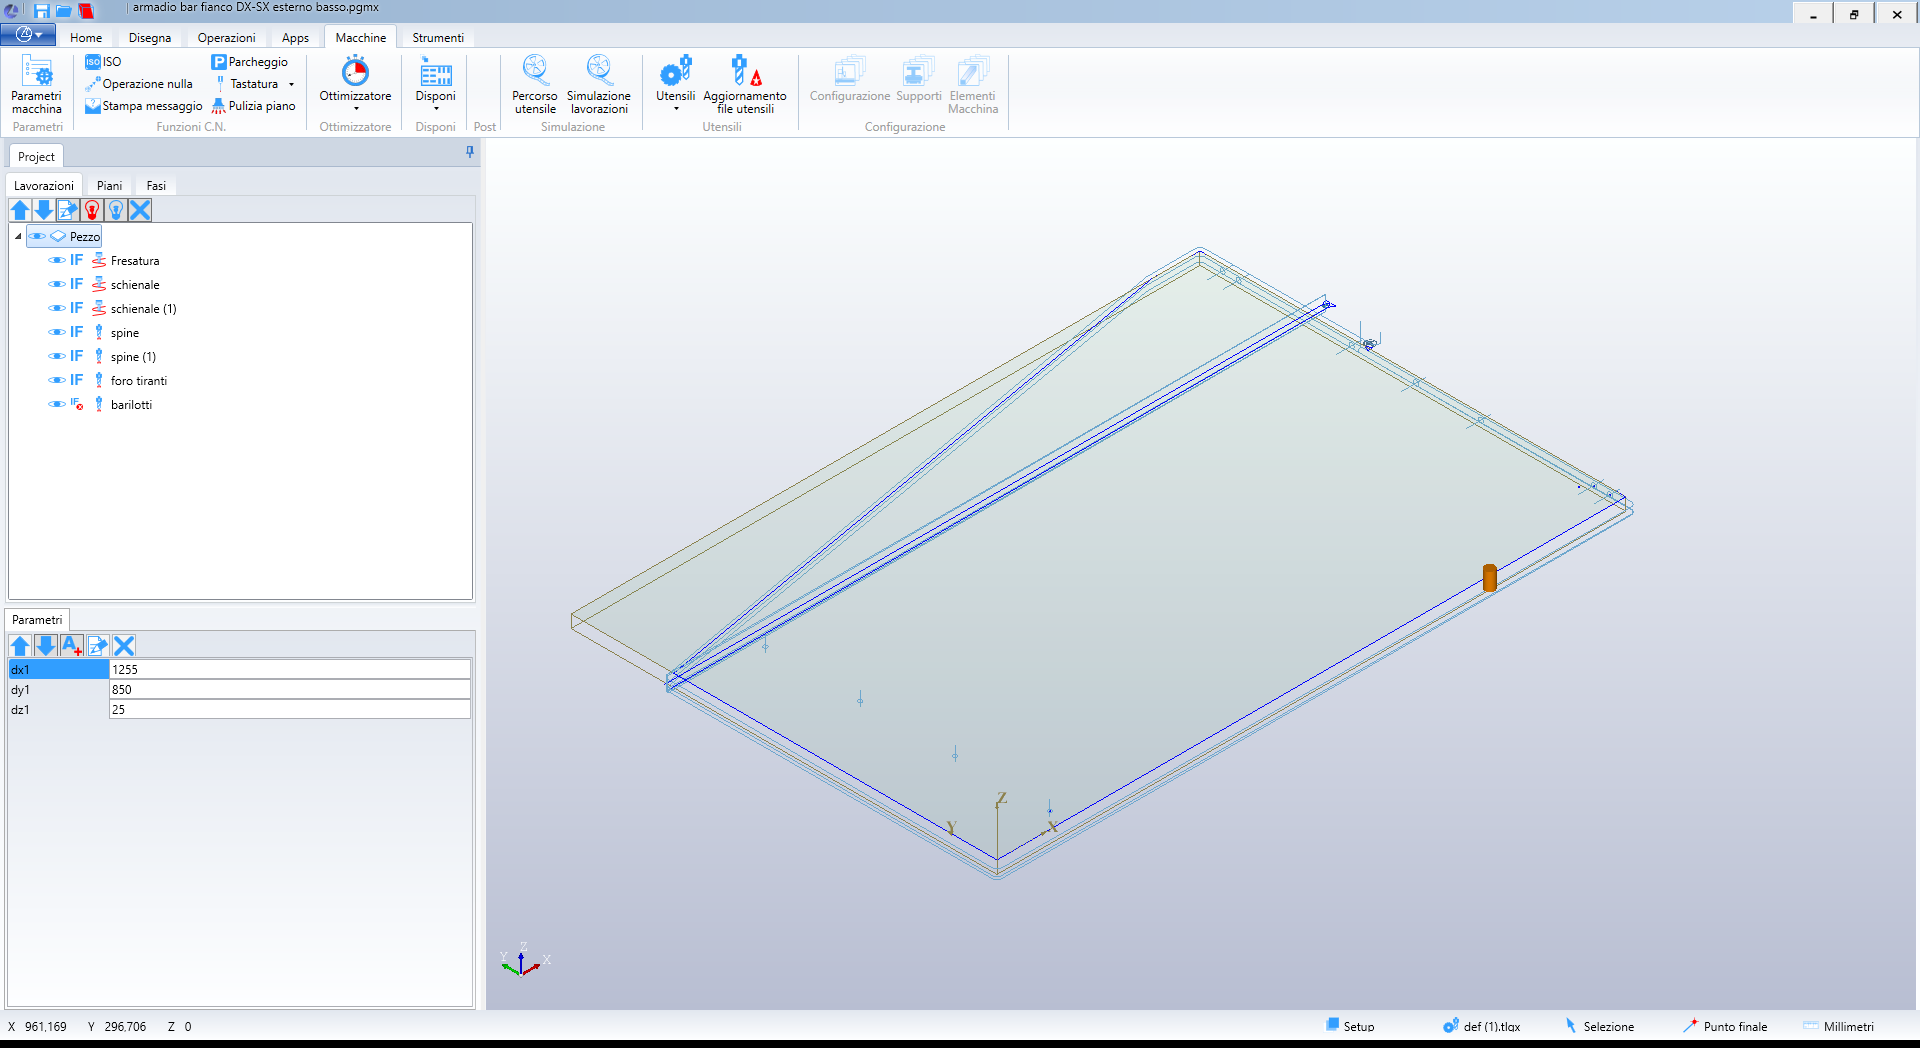
\includegraphics[width=0.8\textwidth]{image28}
	\caption{Programma PGX fianco esterno}
	\label{fig:mesh1}
\end{figure}


\section{Rafforzamento argine ruscello}

Le massicciate e le prismate sono opere di difesa spondale, realizzate con massi e/o con prismi di diverse dimensioni; gli spazi tra essi possono essere liberi o occlusi con cementi di varia natura. 
Sono preferibili le scogliere a secco, senza materiale cementante. Gli spazi permettono una migliore continuità tra fiume e falda; l’eventuale interposizione di geotessuti tra la scogliera ed il terreno retrostante consente il passaggio dell'acqua, limita il trasporto di materiali solidi, ma limita lo sviluppo delle radici delle piante colonizzatrici. 

\begin{figure}[H]
	\centering
	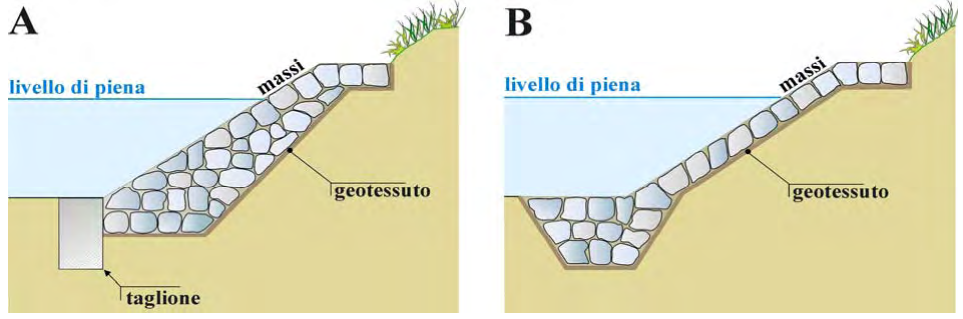
\includegraphics[width=0.8\textwidth]{image36}
	\caption{Sezione fiume}
	\label{fig:spnde}
\end{figure}

Gli spazi consentono la colonizzazione delle piante; ciò limita l’impatto sull'ecosistema e sulla qualità del paesaggio. I vegetali che crescono tra i massi ed i prismi contribuiscono, con le radici, a rendere più stabile le opere e, con le parti aeree, ad assorbire in parte l’energia delle acque di piena. Per accelerare la colonizzazione vegetale, è possibile procedere con impianti artificiali mediante talee o sistemi diversi. \\

\begin{wrapfigure}[14]{r}{0.4\textwidth}
	\centering
	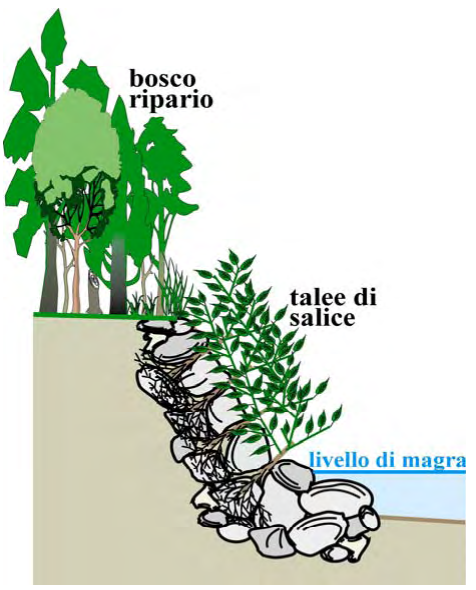
\includegraphics[width=0.3\textwidth]{image27}
	\caption{Sezione fiume}
\end{wrapfigure}

In \cref{fig:spnde} possiamo vedere le difese spondali viste in sezione: scogliera con protezione al piede (A) e mantellata con massi cementati (B).
Tali strutture sono anche denominate “massicciate” e sono caratterizzate da massi di almeno quasi una tonnellata; essi possono essere sostituiti da prismi di cemento. 


La scogliera costituisce una reale difesa puntiforme, ma che trasferisce a valle l’energia di erosione in modo tanto più efficace quanto più regolare è la geometria della scogliera stessa, soprattutto se realizzata con massi e/o prismi cementati.

\subsection{Barriera anti rumore}

Le caratteristiche acustiche di una barriera antirumore possono essere classificate in due categorie: 
\begin{itemize}
	\item estrinseche: efficienza della barriera antirumore nel ridurre i livelli di pressione sonora in una serie di punti sul territorio, chiamati recettori
	\item intrinseche: caratteristiche proprie del “prodotto” barriera antirumore, indipendentemente dall'ambiente in cui è o sarà installato e dall'effetto finale di riduzione del rumore sui ricettori (assorbimento/riflessione, trasmissione, diffrazione del suono).
\end{itemize}


Esistono numerose tipologie di barriere acustiche e di materiali componenti. La scelta di un prodotto dipende, oltre che dalle prestazioni acustiche richieste, anche da fattori, quali: statica, sicurezza, estetica, durata, manutenzione, costi. Le barriere antirumore possono essere suddivise nelle seguenti tipologie: 

\begin{enumerate}
	\item Barriere Artificiali
	\begin{itemize}
		\item Fonoisolanti (struttura alveare)
		\item Fonoassorbenti 
		\item Fonoisolanti e fonoassorbenti
	\end{itemize}
	
	\item Barriere Naturali
	\begin{itemize}
		\item Barriere vegetali (siepi, fasce boscate, alberate) 
		\item Barriere miste (terre armate, biomuri, muri verdi, barriere vegetative)
	\end{itemize}
\end{enumerate}


\subsection{Come l’ho realizzata}

ho deciso di realizzare una barriera antirumore per riparare il chiosco dalla strada molto trafficata, la barriera sarà divisa in due:
La parte esterna, rivolta verso il traffico, sarà realizzata con pannelli in lamiera di acciaio o di alluminio. L'interno dei pannelli ospita uno strato alveolare e un materiale fibroso fonoassorbente che combina attenuazione, isolamento ed assorbimento in una struttura modulare ed economica.
la parte interna, rivolta verso il lago, sarà rivestita dello stesso legno del chiosco. 

\subsection{Allestimento Esterno}

Come tavoli esterni ho deciso di usare le bobine vuote dei cavi, questo perché mi interessa l’arte del riciclo.
Al giorno d’oggi, più che mai, è molto importante utilizzare materiali locali e riciclare tutto quello che possibile.
Il riciclo permette di ridurre gli sprechi e  dare nuova vita ad un prodotto che andrebbe distrutto incrementando il problema dello smaltimento, inoltre permette di limitare l’utilizzo di materiali nuovi. 
Volevo rendere la mia struttura, anche se in minima parte, eco-sostenibile .

\begin{figure}[H]
	\centering
	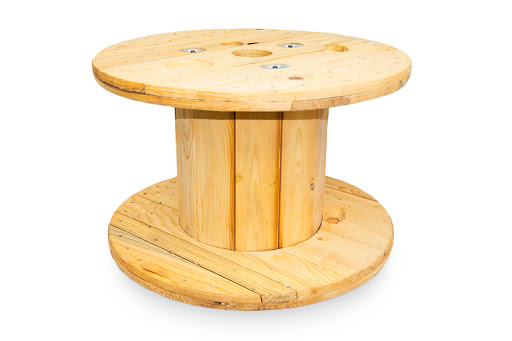
\includegraphics[width=0.8\textwidth]{image3}
	\caption{Bobina}
	\label{fig:mesh1}
\end{figure}



Da una bobina posso ricavare 2 tavoli. 
Ve ne sono di diverse misure, ho scelto quelle da 
$1200 mm$ e $1600 mm$, $H 1500 mm$.

\begin{figure}[H]
	\centering
	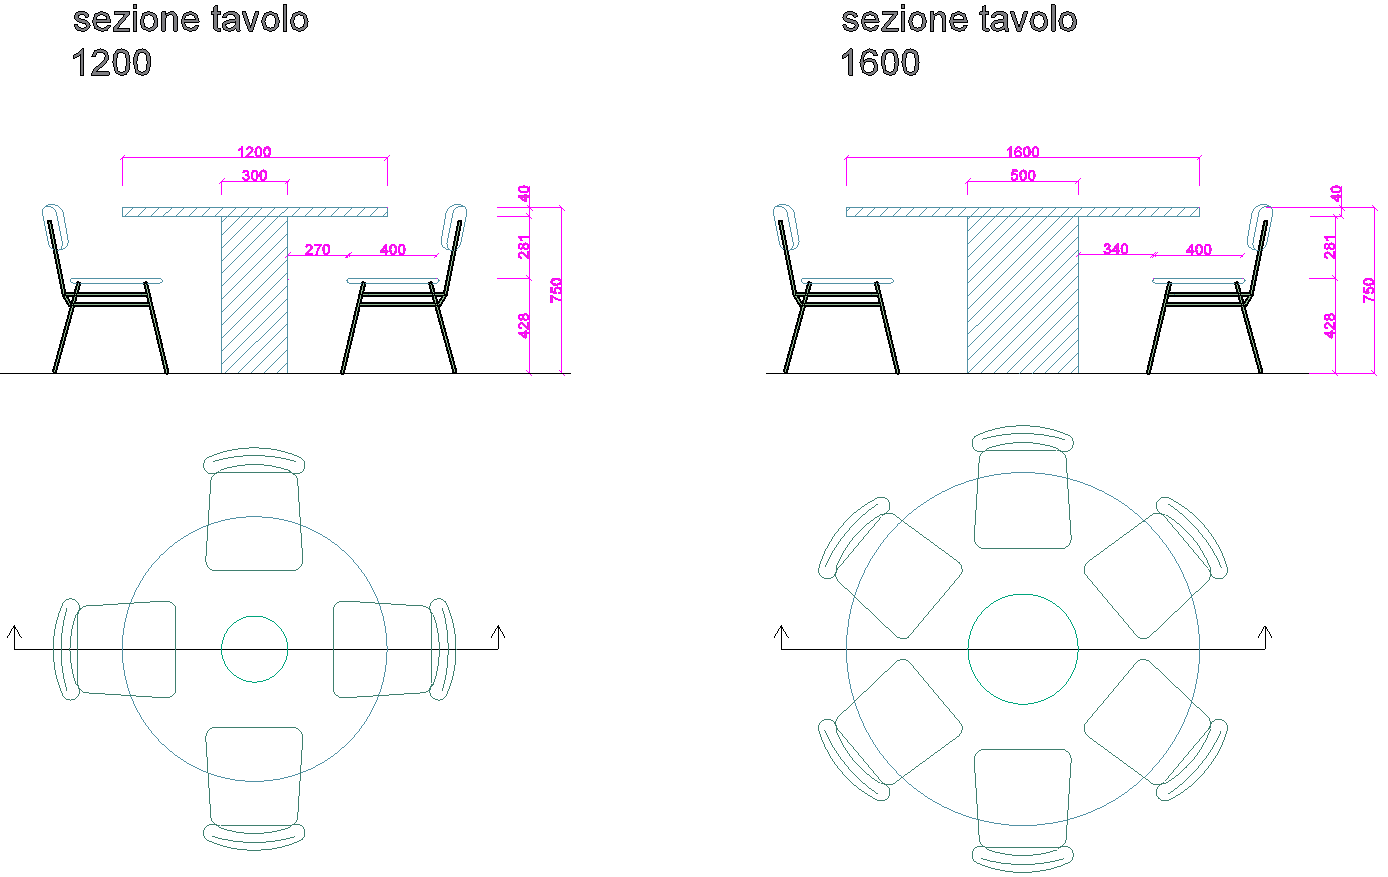
\includegraphics[width=0.8\textwidth]{image31}
	\caption{Sezione tavoli}
	\label{fig:mesh1}
\end{figure}
